\section{Entorno de prueba Mininet}

En el desarrollo de este trabajo, Mininet se ha considerado como uno de los entornos de prueba más relevantes. Su flexibilidad y facilidad de integración lo convierten en una herramienta adecuada para reproducir escenarios de red y evaluar el impacto del sistema de filtrado propuesto en condiciones controladas.

Mininet es un emulador de red que permite diseñar topologías compuestas por hosts finales, switches, routers (aunque de manera no nativa, ofreciendo únicamente el reenvío de paquetes) y enlaces dentro de un único kernel Linux. Además, dispone de una API accesible desde Python, lo que facilita el uso de este lenguaje de programación para la creación y configuración de las topologías de red\cite{lantz2021mininet}.

Como entorno de pruebas, se utilizó Mininet para implementar una topología inicial, que se muestra en la figura \ref{red-mininet-1}. Esta configuración consistía en dos hosts, cada uno conectado a un switch distinto, mientras que ambos switches se encontraban interconectados a un único router. Esta topología permitió realizar pruebas preliminares sobre el impacto del filtro basado en árboles de decisión en el rendimiento de la red.

Si bien esta configuración resultó útil para evaluar el funcionamiento básico del filtro, no era completamente representativa de un escenario real con una tarjeta de red equipada con DPU. Aunque dentro de la tarjeta los paquetes llegan al procesador de la DPU a través de Ethernet, la topología de Mininet no reproduce de manera exacta la interacción de los paquetes con el hardware especializado de la NIC. Al añadir más de una interfaz switch además del router, se introducen latencias adicionales que no existen en la NIC, por lo que este diseño inicial sirve únicamente para pruebas preliminares y no refleja completamente las condiciones de un entorno con DPU.

\begin{figure}[Primera Topología de Red]{red-mininet-1}{Primer diseño de topología de red usada en Mininet preliminares.}
	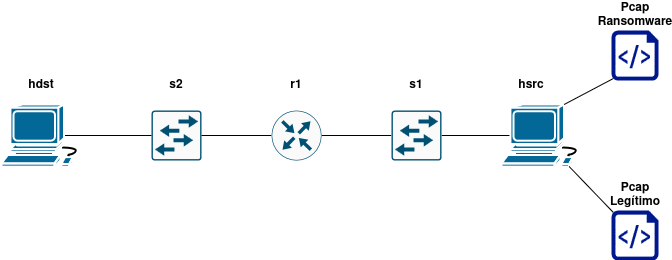
\includegraphics[width=0.9\textwidth]{capturas/DiagramaRedArbol1.png}
\end{figure}

Teniendo en cuenta que el entorno de pruebas real consiste en una tarjeta de red con dos puertos a nivel de enlace, se decidió simplificar la topología de Mininet para realizar pruebas más realistas. La red utilizada consta únicamente de dos host conectados a un único switch, eliminando la necesidad de routers adicionales o interfaces suplementarias tal y como se puede ver en la figura \ref{red-mininet-2}. Esta simplificación permite reducir la complejidad de la topología y minimizar factores externos que podrían afectar a las mediciones, como las latencias introducidas por componentes adicionales de la red virtual.

Además, esta configuración simplificada contribuye a disminuir la pérdida de paquetes durante las pruebas y reduce problemas relacionados con la resolución de direcciones MAC mediante ARP. Al aproximarse más al comportamiento de un entorno real con DPU, la topología proporciona un marco adecuado para medir el rendimiento de la red bajo la influencia del filtro de árbol de decisión. El siguiente paso en el proceso consistirá en realizar pruebas de rendimiento utilizando la herramienta iperf, lo que permitirá cuantificar de manera más precisa el impacto del filtrado sobre el tráfico de red.

\begin{figure}[Topología de Red Final]{red-mininet-2}{Diseño de topología de red usada en Mininet para pruebas.}
	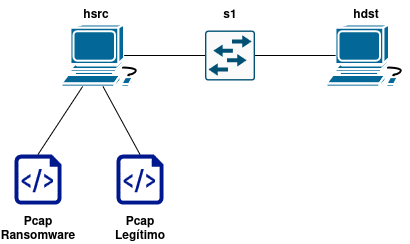
\includegraphics[width=0.55\textwidth]{capturas/DiagramaRed2.png}
\end{figure}

En los fragmentos de código \ref{redarbolrw} y \ref{redarbolrw1} se muestran extractos de los ficheros redarbolrw.py y redarbolrw1.py, correspondientes a la definición de la topología preliminar y de la topología definitiva, respectivamente.

\PythonCode[redarbolrw]{Red Árbol Preeliminar}{Fragmento de códgio que define la topología de red usada en las pruebas preeliminares.}{../Mininet/redarbolrw.py}{22}{54}{22}

\PythonCode[redarbolrw1]{Red Árbol Final}{Fragmento de códgio que define la topología de red usada en las pruebas finales.}{../Mininet/redarbolrw1.py}{8}{25}{8}

\section{Herramientas}

En la presente sección se describen las herramientas empleadas tanto para la generación de tráfico como para la obtención de métricas asociadas. Si bien todas ellas persiguen el mismo objetivo general —evaluar el rendimiento de la red bajo distintas condiciones de carga—, difieren en el tipo de tráfico que generan y en su origen. Esta complementariedad justifica la utilización de las tres, ya que permite llevar a cabo un análisis más completo y ofrecer una visión más precisa del comportamiento del sistema.

\subsection{Iperf}

Iperf 2 es ---como indica su manual\cite{iperf2-manual}--- una herramienta de testeo que emplea sockets de red para realizar medidas de tráfico. Solo acepta los protocolos TCP y UDP, y permite evaluar métricas de rendimiento como el throughput y la latencia. Entre sus funcionalidades se encuentra la posibilidad de generar tráfico unidireccional, full duplex (usando un mismo socket) y bidireccional, además de soportar múltiples flujos simultáneos de manera concurrente. Asimismo, admite tráfico multicast, incluyendo uniones de tipo source-specific multicast (SSM). Su diseño multihilo posibilita alcanzar un rendimiento elevado en las pruebas, mientras que las métricas obtenidas permiten caracterizar el desempeño de la red de extremo a extremo. Para la ejecución de un test es necesario establecer tanto un servidor, que recibe el tráfico, como un cliente, que lo genera y envía; normalmente se ubican en equipos distintos, aunque no es estrictamente necesario.

La elección de Iperf como herramienta de apoyo en la experimentación se justifica principalmente por su simplicidad y facilidad de uso. Esta característica permite diseñar pruebas controladas en entornos ideales, utilizando los dos protocolos de transporte más empleados en la actualidad en el ámbito de las redes, TCP y UDP. Además, la herramienta proporciona de manera integrada métricas fundamentales como ancho de banda, latencia y pérdida de paquetes, las cuales pueden obtenerse bajo diferentes configuraciones sin añadir complejidad al proceso experimental. Gracias a estas propiedades, Iperf resulta especialmente útil para establecer una línea base de rendimiento y evaluar de forma genérica el impacto que introduce el filtro basado en árboles de decisión sobre el tráfico de red.

\subsection{TCPReplay}

TCPReplay es una herramienta diseñada para el reenvío de paquetes de red previamente capturados mediante utilidades como tcpdump o Wireshark. Su principal funcionalidad consiste en reproducir dichos paquetes, bien respetando la velocidad original con la que fueron capturados, o bien a una velocidad definida por el usuario. En este último caso, la herramienta permite ajustar de manera explícita el ritmo de envío, ya sea en función de paquetes por segundo (pps) o de la tasa de transmisión expresada en megabits por segundo (Mbps)\cite{tcpreplay-manpage}.

TCPReplay aporta dos ventajas clave para la evaluación experimental. En primer lugar, permite reproducir tráfico real contenido en ficheros PCAP, lo que posibilita realizar ensayos más representativos que los basados únicamente en tráfico sintético —por ejemplo, incluyendo protocolos distintos de TCP/UDP (ICMP, ARP, SMB, etc.) y secuencias de paquetes reales—. En segundo lugar, ofrece un control fino sobre la velocidad de reproducción (tanto en paquetes por segundo como en Mbps y otras modalidades), lo que facilita la emulación de distintos escenarios de carga de red (desde tráfico esporádico hasta condiciones de estrés). Estas capacidades hacen de TCPReplay una herramienta especialmente adecuada para validar el comportamiento del filtro XDP frente a tráfico heterogéneo y para estudiar su rendimiento bajo diferentes perfiles de carga.

\subsection{Script de Reenvío}

Iperf presenta la limitación de generar tráfico sintético exclusivamente con los protocolos TCP y UDP, lo que resulta insuficiente para el presente trabajo dado que una parte relevante del tráfico legítimo y, de forma más crítica, de las muestras de ransomware emplea otros protocolos (por ejemplo ICMP). En este sentido, Iperf no permite reproducir de forma realista la heterogeneidad de protocolos observada en escenarios reales. Tcpreplay cubre parcialmente esta carencia, ya que posibilita el reenvío de tramas contenidas en ficheros PCAP independientemente del protocolo que utilicen; sin embargo, su operación se limita a reproducir secuencias predefinidas, por lo que no facilita la selección aleatoria en tiempo de ejecución entre tráfico benigno y malicioso, comportamiento que sí sería habitual en un entorno real. Por estas razones se ha desarrollado un script propio que emula un entorno más realista: el generador produce paquetes según la tasa (rate) y la duración especificadas, y para cada envío selecciona aleatoriamente si el paquete será de origen benigno o malicioso, permitiendo además etiquetar cada emisión para su posterior correlación y análisis experimental. Se puede ver un fragmento de la función main del script en el fragmento de código \ref{script_reenvio}, el código completo se encuentra en el fichero \verb|Mininet/trafico_eth.py|.

\PythonCode[script_reenvio]{Script de Reenvío de Paquetes}{Fragmento de códgio del script de reenvío.}{../Mininet/trafico_eth.py}{83}{122}{83}

\subsection{TCPDump}
Tanto TCPReplay como el script desarrollado en este trabajo, a diferencia de Iperf, no disponen de funcionalidades propias para medir el rendimiento de la red, limitándose únicamente al reenvío de paquetes. Por este motivo, resulta necesario complementar su uso con herramientas de captura de tráfico, como TCPDump, que permiten registrar los paquetes transmitidos y analizar posteriormente métricas relevantes como el throughput, la latencia o la pérdida de paquetes\cite{tcpdump-manpage}.

TCPDump es una herramienta de línea de comandos que permite capturar y visualizar paquetes de red en tiempo real. Es capaz de filtrar el tráfico en función de distintos criterios, como direcciones IP, puertos o protocolos, y de guardar las capturas en ficheros para su análisis posterior. Además, TCPDump permite examinar cabeceras de protocolos como Ethernet, IP, TCP y UDP, proporcionando información detallada sobre el flujo de datos entre hosts, lo que lo convierte en un recurso fundamental para evaluar cómo afectan mecanismos de filtrado, como el árbol de decisión XDP, al rendimiento de la red.

\section{Métricas Relevantes}

Para poder analizar el rendimiento del sistema, tanto con el árbol de decisión activo como con este inactivo, es necesario centrarse en una serie de métricas relevantes. Estas métricas permitirán cuantificar de manera objetiva el impacto que el árbol de decisión tiene sobre el comportamiento general del sistema, proporcionando una base sólida para la comparación entre ambos escenarios.

La primera métrica a considerar es el rendimiento o \textit{throughput}, el cual mide la cantidad de información útil que se recibe por segundo. Dado que se trata de un entorno de red, el estándar es expresar esta métrica en bits por segundo (bps) en lugar de utilizar unidades como bytes por segundo u otras equivalentes, ya que permite una representación más precisa y ampliamente aceptada en el ámbito de las comunicaciones de red.

\begin{equation}[eq:throughput]{Cálculo del throughput}
  \text{Throughput (bps)} = \frac{8 \times B_{\text{recibidos}}}{T}
\end{equation}

Además de medir el rendimiento en bits por segundo, resulta de interés cuantificar también el número de paquetes por segundo (PPS) que el sistema es capaz de procesar. Aunque a primera vista esta métrica pueda parecer redundante respecto a la anterior, ambas reflejan aspectos distintos del comportamiento del sistema. En efecto, una misma cantidad total de información puede estar dividida en un número diferente de paquetes, y cada uno de ellos requiere una serie de operaciones de procesamiento que deben ejecutarse de manera independiente --como la lectura de cabeceras, la evaluación de condiciones o el acceso a estructuras de datos internas--. Por este motivo, el rendimiento medido en paquetes por segundo permite identificar posibles cuellos de botella asociados al manejo intensivo de paquetes pequeños y evaluar con mayor precisión el impacto del árbol de decisión sobre la carga computacional del sistema.

\begin{equation}[eq:pps]{Cálculo de paquetes por segundo}
	\text{PPS} = \frac{N_{\text{paquetes}}}{t_{\text{fin}}-t_{\text{inicio}}}
\end{equation}

Otra métrica fundamental en un entorno de red es el porcentaje de pérdida de paquetes (\textit{packet loss rate}). Este parámetro resulta esencial para evaluar la fiabilidad y eficiencia de un sistema, ya que un alto rendimiento en términos de bits por segundo (bps) no necesariamente implica un funcionamiento óptimo si el sistema no es capaz de procesar o asimilar correctamente todo el tráfico recibido. En este sentido, un porcentaje elevado de pérdida puede indicar cuellos de botella, saturación del sistema o limitaciones en la capacidad de procesamiento del tráfico, comprometiendo la eficacia global de la solución.

\begin{equation}[eq:perdida]{Cálculo del porcentaje de pérdida}
  \text{Pérdida (\%)} = 100 \times \frac{N_{\text{enviados}} - N_{\text{recibidos}}}{N_{\text{enviados}}}
\end{equation}

No obstante, la interpretación de esta métrica requiere un análisis diferenciado cuando el filtro basado en el árbol de decisión se encuentra activo. En este caso, parte de los paquetes son descartados de manera intencionada por el propio filtro al ser clasificados como potenciales amenazas. Por tanto, resulta fundamental distinguir entre los paquetes perdidos debido a posibles cuellos de botella generados al añadir una nueva capa de procesamiento y aquellos paquetes que son eliminados de manera deliberada por el filtro como parte de su funcionamiento normal. Esta distinción permite evaluar con precisión tanto la eficiencia del sistema como la eficacia del mecanismo de filtrado implementado.

\begin{equation}[eq:perdida arbor]{Cálculo del porcentaje de pérdida con árbol activo}
  \text{Pérdida Real(\%)} = 100 \times \frac{N_{\text{enviados}} - N_{\text{recibidos}} - N_{\text{filtrados}}}{N_{\text{enviados}}}
\end{equation}

\section{Metodología Seguida}
